%; whizzy chapter
% -initex iniptex -latex platex -format platex -bibtex jbibtex -fmt fmt
% 以上 whizzytex を使用する場合の設定。

%     Tokyo Debian Meeting resources
%     Copyright (C) 2007 Junichi Uekawa

%     This program is free software; you can redistribute it and/or modify
%     it under the terms of the GNU General Public License as published by
%     the Free Software Foundation; either version 2 of the License, or
%     (at your option) any later version.

%     This program is distributed in the hope that it will be useful,
%     but WITHOUT ANY WARRANTY; without even the implied warranty of
%     MERCHANTABILITY or FITNESS FOR A PARTICULAR PURPOSE.  See the
%     GNU General Public License for more details.

%     You should have received a copy of the GNU General Public License
%     along with this program; if not, write to the Free Software
%     Foundation, Inc., 51 Franklin St, Fifth Floor, Boston, MA  02110-1301 USA

%  preview (shell-command (concat "xpdf " (replace-regexp-in-string "tex$" "pdf"(buffer-file-name)) "&"))
% 画像ファイルを処理するためにはebbを利用してboundingboxを作成。
%(shell-command "cd image200704; ebb *.png")

%%ここからヘッダ開始。

\documentclass[mingoth,a4paper]{jsarticle}
\usepackage[dvipdfmx]{graphicx}
\usepackage{fancybox}
\usepackage{longtable}
\usepackage{ascmac}	% 囲み (screen,itembox)
\usepackage{fancyvrb}   % 囲み Verbatim のために必要
\usepackage[dvipdfmx]{hyperref}
\usepackage{url}
\usepackage[dvipdfmx]{color}
\usepackage{nextpage}
\usepackage{wrapfig} 

% 日付を定義する、毎月変わります。
\newcommand{\debmtgyear}{2007}
\newcommand{\debmtgdate}{21}
\newcommand{\debmtgmonth}{4}
\newcommand{\debmtgnumber}{27}

%http://www.naney.org/diki/dk/hyperref.html
%日本語EUC系環境の時
\AtBeginDvi{\special{pdf:tounicode EUC-UCS2}}
%シフトJIS系環境の時
%\AtBeginDvi{\special{pdf:tounicode 90ms-RKSJ-UCS2}}

%% spacing の設定をする。外枠を減らす。
\setlength\headheight{0mm}
\setlength\topmargin{-20mm}
\setlength\headsep{0mm}
\setlength\topskip{3mm}
\setlength\maxdepth{4pt}
\setlength\columnsep{6mm}
\setlength\textheight{252mm}
\setlength\topmargin{-5mm}
\setlength\textwidth{170mm}
\setlength\oddsidemargin{-5mm}
\setlength\evensidemargin{-5mm}

% commandline環境を定義。画面入出力についてはcommandline環境
% で表記する
\newenvironment{commandline}%
{\VerbatimEnvironment
  \begin{Sbox}\begin{minipage}{15cm}\begin{fontsize}{7.3}{7.3} \begin{BVerbatim}}%
{\end{BVerbatim}\end{fontsize}\end{minipage}\end{Sbox}
  \setlength{\fboxsep}{8pt}\begin{itembox}[c]{出力}{\TheSbox}\end{itembox}}


%%% start of santaku
\makeatletter
\newwrite\tf@jqz
\immediate\openout\tf@jqz\jobname.jqz\relax
\makeatother
\newcounter{santakucounter}
\newcommand{\santaku}[5]{%
\addtocounter{santakucounter}{1}

\addtocontents{jqz}{\arabic{santakucounter}. #5\\}
\begin{minipage}{1\hsize}
問題\arabic{santakucounter}. 
#1\\
□ A #2\\
□ B #3\\
□ C #4
\end{minipage}
\hspace{1cm}
\\

}
%%% end of santaku

\newcommand{\emptyspace}{(\underline{\hspace{1cm}})}

\newcommand{\subsubsubsection}[1]{%
\vspace{1zw}{\bf #1}\\}


% sectionをセンタリングする
\makeatletter
  \renewcommand{\section}{\@startsection{section}{1}{\z@}%
    {\Cvs \@plus.5\Cdp \@minus.2\Cdp}% 前アキ
    {.5\Cvs \@plus.3\Cdp}% 後アキ
    {\normalfont\gt\fontsize{32}{32}\headfont\raggedright}} % style
\makeatother

% section の代わりの環境
\newcommand{\dancersection}[2]{%
\newpage
第\debmtgnumber{}回 東京エリアDebian勉強会 \debmtgyear{}年\debmtgmonth{}月
\hrule
\vspace{0.5mm}
\hrule
%
\vspace{4cm}
\hrule
\vspace{0.5mm}
\hrule
%
\vspace{-7cm}
\begin{minipage}[b]{0.7\hsize}
\section{#1}
\hfill{}#2\\
\vspace{2cm}
\end{minipage}
\begin{minipage}[b]{0.3\hsize}
\hfill{}
\includegraphics[height=8cm]{image200502/openlogo-nd.eps}\\
\end{minipage}
%
%\hfill{}
\includegraphics[width=16cm]{image2006-natsu/guruguru-sand-light.png}\\
\vspace{-1cm}
}

% BTSの番号を見るためのコマンド
\newcommand{\debianbug}[1]{Bug\##1\footnote{\url{http://bugs.debian.org/#1}}}

% for dancerj
\newcommand{\fgref}[1]{図\ref{#1}}
\newcommand{\tbref}[1]{表\ref{#1}}

\begin{document}


\begin{titlepage}

 第\debmtgnumber{}回 東京エリア Debian 勉強会資料

\vspace{2cm}

\begin{minipage}[t]{0.6\hsize}
\vspace{-2cm}
{\fontsize{60}{60}
{\gt
東京エリア \\
デビアン \\
勉強会
}}
\end{minipage}
\begin{minipage}[b]{0.4\hsize}
\hspace{-1cm}
\includegraphics[width=9cm]{image200502/openlogo-nd.eps}
\end{minipage}

\vspace{3cm}
\hfill{}Debian勉強会幹事 上川 純一\\
\hfill{}\debmtgyear{}年\debmtgmonth{}月\debmtgdate{}日

\thispagestyle{empty}
\end{titlepage}

\dancersection{Introduction}{上川 純一}
 
 今月のDebian勉強会へようこそ。
 これからDebianのあやしい世界に入るという方も、すでにどっぷりとつかってい
 るという方も、月に一回Debianについて語りませんか?

 目的として次の二つを考えています。

 \begin{itemize}
 \item メールではよみとれない、もしくはよみとってられないような情報につ
       いて情報共有する場をつくる
 \item Debianを利用する際の情報をまとめて、ある程度の塊として整理するた
       めの場をつくる
 \end{itemize}

 Debianの勉強会ということで究極的には参加者全員がDebian Packageをがりがり
 と作るスーパーハッカーになった姿を妄想しています。

 Debianをこれからどうするという能動的な展開への土台としての空間を提供し、
 情報の共有をしたい、というのが目的です。


\newpage

\begin{minipage}[b]{0.2\hsize}
 \definecolor{titleback}{gray}{0.9}
 \colorbox{titleback}{\rotatebox{90}{\fontsize{80}{80} {\gt デビアン勉強会} }}
\end{minipage}
\begin{minipage}[b]{0.8\hsize}
\hrule
\vspace{2mm}
\hrule
\tableofcontents
\vspace{2mm}
\hrule
\end{minipage}

\dancersection{事前課題}{上川 純一}

今回の事前課題は
「私はバージョン管理システムをこのようにつかっています」もしくは「バージョン管理システムを使わなくてすむようにこのようにしています」
というタイトルで200-800文字程度の文章を書いてください。というものでした。
その課題に対して下記の内容を提出いただきました。

\subsection{青木さん}

VCSはCVSとSVNを使っていますが、あまり複雑なパッチ管理ではなく
単に共同開発の最新版管理レベルです。それとバックアップ的な意
味合いで使います。ハンドマージより凝ったことといえばVIMDIFの
利用ぐらいがせいぜいです。タグ管理はとくいではないです。DVCS
をつかうべきかと思いつつ、勉強不足ですね。

\subsection{Kentaro Wakiさん}
\subsubsection{私はバージョン管理システムをこのようにつかっています}

特に変わった使いかたはしていません。
一応、プログラマなのでソースコードのバージョン管理に「subversion」使ってます。
つい最近まで「CVS」使ってました。
「subversion」で気に入ったのは、「ファイル名の変更」「ブランチの扱い」などです。また、「windows」ユーザと連係する場合に便利そうに見えます。
まだ実際には触ってませんが、「TortoiseSVN」は「windows」ユーザに違和感の少ないUIっぽいので。
「subversion」関連で、「Trac」の評判も良いようなので導入を検討しています。

\subsection{森田尚さん}

\subsubsection{私はバージョン管理システムをこのようにつかっています}

個人で余暇に書いているプログラムのソースコード管理と、仕事(出版社で書籍
の企画・編集をしています)での原稿管理のために、Subversionリポジトリを
Apacheでホストして使っています。2002-2004年ごろは主にCVSを使っていました。

自分の仕事では、協働するチームメンバが複数の組織と拠点に分散していること
が多いので、いずれ分散型VCSを導入したいと考えています。

\subsubsection{バージョン管理システムを使わなくてすむようにこのようにしています}

数世代にわたるバックアップが欲しいだけのときなど、VCSを使うまでもない場
合のために、ホームディレクトリその他をpdumpfsのバックアップ対象にしてい
ます。

\subsection{akeさん}

「バージョン管理システムを使わなくてすむようにこのようにしています」
何故バージョン管理システムが必要なのか?
一つの物に複数でよってたかって改変を加えるからである。
であれば、使わなくて済むようにするアプローチとして
\begin{itemize}
 \item 複数の改変を同時にしない
 \item 複数の改変が相互に影響しないようにする
\end{itemize}

のどちらかを行えば良いのである。
前者は改変を一人が行うと言う事になるが現実的ではない
後者を実現するためには、設計プロセスが完全でなければならない
要するに、ソフトウェア開発であれば、
モジュール化が適切に行われているなど、
設計の瑕疵を無くせばバージョン管理システムは不要である。
と言う事に行き着く。
実際の所、そう言った状況で作られるソフトウェアはまず無い。
多くの開発現場では、混沌の中から偶然の産物の様に作り出されたりする。
この状況が存在する限り、やはりバージョン管理システムは必要とされ続けるのだろう。
だが設計プロセスを注意深く行えば、設計プロセスの瑕疵を無くす手法が見つかれば、
なんとか実現できるかも知れない。

\subsection{Hashimoto, Toruさん}

  今のソフトウェア開発プロジェクトでは、何とバージョン管理システムを使っ
ていない。複数の人が同じファイルを編集しようとすることも実際にあり、そ
の状況はかなり問題である。プロジェクト全体としてバージョン管理を導入す
る考えはないようである。そこで、自分のチーム内で独自にソースコードを管
理する方式を考えているところである。

  使用するツールとしてはSubversionを考えている。チームの担当範囲のファ
イルは決まっているので、バージョン管理対象は明確ではあるが、開発環境が
よく言えば特殊、悪く言えば洗練されていないために実際にきれいに適用する
のは一筋縄ではいかない。こんな環境でもうまく運用できる方法を考えている
ところである。

  その他、自分だけではあるがパッチ管理としてquiltを使ってみたことがあ
る。自分の変更点をパッチ(diff)にするのが自動的にできるのは便利だが、自
分の作業中に他人が同じファイルを編集するということが起こると混乱してし
まった。こういう用途には向かないようだ。


\subsection{Noriaki Sato}

私はバージョン管理システムをこのようにつかっていたり、
いなかったりします(しました)

一年前まで:\\
バージョン管理システムを使ったことがありませんでした。
当時は、実験データ解析用のコードを書いていましたが、
\texttt{hoge\_{}20051204.cc} のようなファイル名だけで管理していました。
(頻繁に書き直したりするわけじゃないので、それで済んでいた)
CVS とか名前は知っていたけど、覚えている余裕がありませんでした。

一年前:\\
仕事で初めて VSS を使いました。
チェックアウトするとロックされてしまうのが不便じゃね?
と思いました。その後、VSS に上げる前のソースコードを
自分のローカルマシン上で管理するために Subversion を使っていました。
「達人プログラマ」で、ソースコード以外の普通のドキュメントも
バージョン管理システムで管理しよう、と言う話を読んで、
なるほど!と思いましたが、結局、今に至るまで実践はしていません。

今:\\
今度の現場では VSS を使わせてくれないらしいです。
それほどコードを書く必要のないプロジェクトなのですが、
台帳で管理するとか言う話です。
フリーソフトのインストールも不可なので、
svn を入れて使ったりする事も出来ません。
(一番つらいのは emacs(meadow) を使えない事なのですが、オフトピですね)


\subsection{鈴木さん}
バージョン管理は、cvsとsubversionを使ったことがあります。
cvsは、Web(tlec.linux.or.jp)の更新で利用しています。チェックアウトすれば
どこでも更新
できるので便利です。最近余り更新してませんが。
subversionは、ドキュメント作成を会社と家で更新できるような1日の区切りで
チェックイン
していました。使ったり使わなかったりで持続しないです。理由は、リリースす
るときにtarに
まとめてバックアップしているので頻繁にsubversionは使ってないです。


\subsection{H.Honjoさん}
個人で管理しているサーバに、バージョン管理システムとして
Subversionを、バグトラックシステムにはtracを利用しています。特に
変わった用途として使ってはおらず、通常どおりソースコード管理およ
びバグトラックとして使用しています。主にクライアントマシンとして
Windowsを使用している関係から、TortoiseSVNをSubversionのクライア
ントとして利用しています。

新たにリリースされたEtchへの移行を検討しており調査中ですが、
trac-ja-resourceパッケージがうまく動作してくれず、難航しています。

\subsection{小室 文さん}
\subsubsection{バージョン管理システムを使わなくてすむようにこのようにしています}

バージョン管理は使っていません。会社ではバージョン管理を使うような人や案件はないです。
プライベートでも管理する物も一緒に管理したい人もいないので、導入していません。

バージョン管理を導入する場合、使う人が対等な位置にいるのが前提な気がします。なので、他の案件の一部分の機能を追加するためにファイルを検証サーバにアップする際は(1)事後報告するか(2)案件管理者にファイルを送る事が多いです。

使ってみないと!と思いつつも必要に迫られていないのでよく理解していません。


\subsection{北原さん}

\subsubsection{バージョン管理システムを使わなくてすむようにこのようにしています}


回答:\\
個人的に作成しているプログラムはたいした量ではないので、「使わ
なくてすむように」というよりは、「使う必要がない」という状態です。  

プログラムを構成するファイルは、修正前にファイル名にバージョン番号を付け
て、全バージョンそのままの形で保存してあります。(若しくは、ディレクトリ
にバージョン番号を付けて丸ごとコピー。) 規模が小さいのでこれで十分管理
できてしまいます。

\subsection{小林儀匡}

「私はバージョン管理システムをこのようにつかっています」

内容が日々進化していくファイル (プログラム・ドキュメント・翻訳・図など) 
は何でもリポジトリに入れてバージョン管理下に置いています。バージョン管
理システムのない生活はもう考えられなく、バージョン管理システムがあって
こそ効率的な仕事ができると思うようになっています。

これまでは主にSubversionなどの中央集権的なバージョン管理システムしか使っ
てきませんでしたが、最近、Debianのウェブサイトやリリースノートの日本語
訳コーディネータとして働くようになってから、分散バージョン管理システム
にも興味をもつようになりました。翻訳チーム全員にコミット権を与えるわけ
にはいかないというのはプロジェクトとしては仕方がないことだと思いますが、
他方でコーディネータとしては、あらゆるコントリビュータの仕事はきちんと
区別し、分割してコミットしたいのです。しかしそのような作業をコーディネー
タ一人でやるのは大変なので、分散バージョン管理システムを導入して、本家
リポジトリへのコミット権はもっていなくても自分のリポジトリにコミットで
きる翻訳者やレビューアにはどんどん自分で作業をしてもらったほうが、効率
がいいのではないかと思っています。

\subsection{えとーさん}

\subsubsection{私はバージョン管理システムをこのようにつかっています}


自前のソースコードの管理や参加しているプロジェクトのソースコードの管理に
利用しています。

設定ファイルやその他雑多なものはあまり利用できていないので、今後も勉強しながら
便利に使っていきたいと思っています。


\subsection{keng nakさん}

バージョン管理システムは、仕事で cvs をつかっています。ソー
スコードから word や excel の資料からメモに至るまですべて
まとめて cvs で管理していました。
今度配属されたプロジェクトでは Mercurial(OpenSolarisなど
で採用されている分散SCM)を使用することになり、今まで使っ
てきた cvs とは勝手が違うために戸惑っております。
今回は分散SCMが2種類紹介されるようですので、この機会に
分散SCMの有効な使い方を学べたらと思っています。
よろしくお願いします。


\subsection{でん@相模原さん}

従来、自作プログラムは環境情報をまとめたメモと一緒にソース
ファイル一式をtar.bz2で固めて蓄積してました。

この方法ではソースを管理すると言う点では問題は無いのですが
それ以外への発展が無く、方々の作業で無駄が発生しました。
代表的なのが、差分抽出により目的外の変更が入っていない事の
確認です。このような事をサポートしてくれるツールとして
バージョン管理ツールのDIFF機能を利用しています。

またバージョン管理業務を長く行っていると
\begin{itemize}
 \item   「何故バージョンを更新したのか」とか
 \item   「どうして、このような作りになっているのか」
\end{itemize}
といった事が忘れてしまいがちです。
このためバグトラッキングシステム(Trac)や自動ドキュメント化
システム(Doxygen)等との連携が今後の課題になっています。

今回のお題にはあがりませんでしたが、私は以下のようなシステム
で個人的には作業をしています。

\begin{itemize}
 \item バグトラッキング、仕様書管理
   → Trac
 \item バージョン管理
   → SubVersion/SVK
\end{itemize}

%%% trivia quiz
\dancersection{Debian Weekly News trivia quiz}{上川 純一}

ところで、Debian Weekly News (DWN)は読んでいますか?
Debian 界隈でおきていることについて書いているDebian Weekly News.
毎回読んでいるといろいろと分かって来ますが、一人で読んでいても、解説が少
ないので、
意味がわからないところもあるかも知れません。みんなでDWNを読んでみましょう。

漫然と読むだけではおもしろくないので、DWNの記事から出題した以下の質問にこたえてみてください。
後で内容は解説します。

\subsection{2007年04号}
\url{http://www.debian.org/News/weekly/2007/04/}
にある3月13日版です。

\santaku
{ウェブアプリケーション関連のパッケージの静的コンテンツはどこにおくべきか?}
{/var/www に置く}
{/usr/share/PACKAGE に置く}
{/srv/XXX に置く}
{B}


\santaku
{Debian Projectの MIA アカウントに対して 実施するWaTとは何をするもの
か}
{今年のDPL選挙に投票しなかった人に対して確認メールを送り反応がない人を引
退プロセスに移行する}
{気に入らない人を強制退会させる}
{あれ?Debian Developerだらけの水泳大会}
{A}

\santaku
{etch リリースはどういう暗号鍵で署名されるか?}
{オンライン鍵とオフライン鍵}
{オフライン鍵のみ}
{オンライン鍵のみ}
{A}

% オンライン鍵は、ネットワーク上にオンラインになっている鍵で、自動処理
%するためにパスフレーズすらない。

\santaku
{Frans PopがアナウンスしたBabelboxは何をするものか?}
{いろいろな言葉を喋ってくれる}
{フォントを複数表示}
{自動でくりかえし Debian Installer が稼働し、Gnomeにしばらくログインしてくれるしく
み}
{C}

\santaku
{DPL選挙の勝者は?}
{Iwamatsu}
{Sam Hocevar}
{Anthony Towns}
{B}

\dancersection{最近のDebian関連のミーティング報告}{上川 純一}

\subsection{東京エリアDebian勉強会25回目報告}
% (query-replace-regexp "<.*>" "")


東京エリアDebian勉強会報告。2月の第25回Debian勉強会を実施しました。今回
は初の小林さんが幹事の会の予定でしたが、小林さんがたおれてしまったので、
代理開催です。

今回の参加人数は13人でした。あけどさん、小室さん、岩松さん、えとーさん、
上川、吉田さん@板橋、Henrichさん、前田さん、石原さん、David Smithさん、
澤田さん、キタハラさん、吉田さん(女性)でした。

上川が最近の事情の紹介、事前課題の紹介をしました。「apt に足りない機能」
という話題では、非常に盛り上がりました。インストールする前に changelog 
や README や manpage を表示するためのインタフェースや、google と連携し
てパッケージをインストールできるようにするインタフェースなどがあるといい
ね、という話題が出ました。また、ユーザのホームディレクトリにインストール
したパッケージもシステム全体の観点から管理できるとよいねという話題も出ま
した。

DWNクイズはひさしぶりにDWNが頻繁にリリースされたので、11問ありました。
みなさまのDebianについての常識を問いました。よい感じですね。

dbs について岩松さんが紹介しました。
dpatch, quilt によって置き換えられつつあるdbsですが、まだ使っているところもあるので抑えておく必要があります。
癖のあるツールですが、この話を聞いてもうみなさん大丈夫ですよね。

そして、上川がdpatch について話をしました。ツールがどういう使い方になる
のか、ということと、一つ dbs 風にも使えるのだ、という事例を紹介しました。

最後に、OSCでの出し物に付いて議論しました。仮想化については、みなさんす
でに活用しまくっているようで、おもしろい話がきけました。Debianユーザじゃ
ない人たちもくるだろうけど、そういう場合にはWindowsからDebianに安心して
乗り換えてもらえるようにgoodbye-microsoft.com を紹介しましょう、という話
をしました。仮想化の使い道としておもしろいものとして、年賀状、EDYチャー
ジ、winny、試験用(教育)などの事例が出てきました。

\subsection{東京エリアDebian勉強会26回目報告}
% (query-replace-regexp "<.*>" "")

オープンソースカンファレンス(OSC)への仮想化友の会と、東京エリアDebian勉
強会参加報告。3月の第26回Debian勉強会を実施しました。今回は仮想化友の会
と共催でOSCの会場で開催します。

今回の参加人数は80人程度でした。

セミナー会場でのオープニングは仮想化友の会の紹介を平さん、Debian勉強会の
紹介を上川がしました。これでみんな勉強会に参加できるようになったと思いま
す。よろしくおねがいします。

事前課題の声を紹介しました。今回の課題は「仮想化を実際にこういう利用方法
で活用しています」でした。さまざまなおもしろい実用例を紹介しました。会場
でもそういう使いかたしている、という声が聞こえてきました。別のアーキテク
チャのエミュレータを活用して開発だとかカーネルの開発に利用しているという
声はあまり聞こえずその利用方法はまだマイナーなようです。

今回はDebian weekly news クイズではなく、「仮想化常識クイズ」を実施しま
した。全員起立願い、クイズの回答を「グー」「チョキ」「パー」で答えてもら
い、正解した人だけのこるという形式でやりました。でんさんが最後まで正解し
ました。おめでとうございます。

山根さんが「Windowsから見える仮想化世界」の紹介をしてくれました。仮想化
技術の現状を紹介、でもWindowsを使うよりも goodbye-microsoft.com を利用し
て Debian をインストールしたほうがよいよ、という紹介でした。Debian勉強会
の趣旨に沿った素晴らしい発表です。

今回のメイントピックとして、前田さんにKVMとの出会いと活用について語って
いただきました。各種OSを稼働したりした例を紹介しました。

その後はどんどんマニアックな内容に突入します。平さんが「私はこれで○○を
辞めました」という発表をしました。素敵な内容でした。

KVMの利用例の紹介として、上川が「KVMでgoodbye-microsoft.comを試す」
「PaSoRiを試す」実演をしました。

平さんが最後にKVMのソースを読んで解析してみるネタを披露しました。これで
もうみんなKVMの起動部分についてハックできるようになったはず。

仮想化友の会とDebian勉強会はブースもかまえていました。ミニセミナーで、山
根さんが自分でパッケージングしたソフトウェアの利用方法を紹介するべく、
「2chリーダーJDの使いかた実演」をしました。

上川が「realcsh, realksh」の紹介をしました。プレゼンテーションは、
realksh で 「panic()」するところで終了しました。

懇親会はイタリアンカフェで。あと、一部でベトナム料理を食べにいきました。
ふー、長い一日でした。

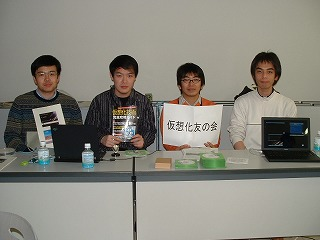
\includegraphics{image200704/DSCF0063.jpg}
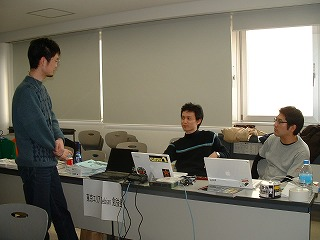
\includegraphics{image200704/DSCF0064.jpg}


\dancersection{darcs 使いかた}{David Smith}
\label{sec:darcs}


darcsはソースコード管理ツールの一つです。Haskellで開発されている注目プロ
ジェクトとしてEmacs、Common Lisp、そしてHaskellのコミュニティでは大好評で
す。\footnote{大好評は多分言い過ぎます。せいぜい部分的に気に入られていま
す。}

git、Mercurial、monotone、他の数多くの分散ソース管理ツールの仲間であ
ります。しかし、gitなどの分散ソース管理ツールと違い、バージョンは管理しな
く、パッチを管理します。その二つの理念の違い、つまりバージョン管理対パッ
チ管理、についてdarcsを活用しながら説明します。

\subsection{基本なdarcs}

\subsubsection{とりあえず使ってみよう}

先ず、新規リポジトリを作ってみます。

\begin{commandline}
exponent,1102:~/workspace> mkdir myproject
exponent,1103:~/workspace> cd myproject
exponent,1104:~/workspace/myproject> darcs ini
exponent,1105:~/workspace/myproject> ls
_darcs
exponent,1106:~/workspace/myproject> echo 'Hello Darcs!' > README
exponent,1107:~/workspace/myproject> darcs whatsnew
No changes!
exponent,1108:~/workspace/myproject> darcs add README
exponent,1109:~/workspace/myproject> darcs whatsnew
\{
addfile ./README
hunk ./README 1
+Hello Darcs!
\}
exponent,1110:~/workspace/myproject> darcs record
Darcs needs to know what name (conventionally an email address) to use as the
patch author, e.g. 'Fred Bloggs <fred@bloggs.invalid>'.  If you provide one
now it will be stored in the file '_darcs/prefs/author' and used as a default
in the future.  To change your preferred author address, simply delete or edit
this file.\footnote{残念ながら、国際化はまだまだ出来ていません。}

What is your email address? David Smith <davidsmith@acm.org>
addfile ./README
Shall I record this change? (1/?)  [ynWsfqadjkc], or ? for help: y

hunk ./README 1
+Hello Darcs!
Shall I record this change? (2/?)  [ynWsfqadjkc], or ? for help: y

What is the patch name? Say hello to darcs
Do you want to add a long comment? [yn]n

Finished recording patch 'Say hello to darcs'
exponent,1111:~/workspace/myproject> darcs changes
Fri Apr 20 15:43:45 JST 2007  David Smith <davidsmith@acm.org>
  * Say hello to darcs
\end{commandline}

darcsではリポジトリの状態はパッチ集合だけで成り立ちます。パッチ
を作るのはファイルをdarcsに登録し、内容を記録し、最後に名前付けで完成し
ます。ちなみにパッチは名前だけで識別され、バージョン番号は一切ありません。
\footnote{自分の名前とメール先を\$HOME/.darcs/authorに書いたら聞かれませ
ん。}

\begin{tabular}{|l|l|p{15em}|l|}
\hline
\hline
コマンド名 & 例 & 意味\\
\hline
init & darcs init & 
 リポジトリを初期化する\\
\hline
whatsnew & darcs whatsnew -v &
 現在のリポジトリと記録済みの情報との差分を明示する\\
\hline
record & darcs record -m 'バグ\#103を修正' &
 パッチをリポジトリに記録する\\
\hline
changes & darcs changes --summary &
 パッチによるチェンジログを生成する\\
\hline
add & darcs add realcsh.c &
 新しいファイルをdarcsに教える\\
mv & darcs mv realcsh.c dangershell.c &
 ファイル名前変更\\
\hline
\hline
\end{tabular}

\subsubsection{他のリポジトリとの同期}

darcsはリポジトリ内のブランチをサポートしてません。複数リポジトリに同じパッ
チを一個も共有すれば、ブランチと呼んでもいいとのことです。つまり、リポジ
トリのコピーしかブランチが作れません。darcs getで既に存在するロカールリポ
ジトリ又はネットワークを通して取得出来るリポジトリでコピーできます。
\footnote{現在、HTTP及びSSHのみの通信になっています。}もちろん、ローカル
の場合にgetを使わずcpでも大丈夫です。

\begin{commandline}
exponent,1049:~/workspace> darcs get myproject myproject2
Copying patch 1 of 1... done!
Finished getting.
exponent,1050:~/workspace> cd myproject2
exponent,1051:~/workspace/myproject2> echo 'Darcs rules!' >> README
exponent,1052:~/workspace/myproject2> darcs record -m 'Add more darcs love'
hunk ./README 2
+Darcs rules!
Shall I record this change? (1/?)  [ynWsfqadjkc], or ? for help: y

Finished recording patch 'Add more darcs love'
exponent,1054:~/workspace/myproject2> darcs push ../myproject

Fri Apr 20 18:04:37 JST 2007  David Smith <davidsmith@acm.org>
  * Add more darcs love
Shall I push this patch? (1/1)  [ynWvpxqadjk], or ? for help: y

Finished applying...

exponent,1055:~/workspace/myproject2>
\end{commandline}

この時、先方のリポジトリに書き込み権利がありましたが、公開されている一般
的なプロジェクトでは開発者以外はコミット出来ませんでしょう。そのため、
push/pullの代わりにsend/applyを使います。sendは指定するパッチをメールで送
り、applyはファイルにあるdarcs形式パッチをリポジトリに記録。

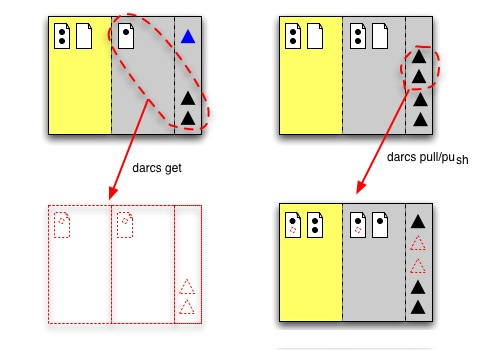
\includegraphics{image200704/darcs/pushpull.jpg}

ここまでdarcsの機能がほとんど普通だと言えますでしょう。しかしながら
パッチとパッチの依存関係を計算するための「パッチ代数」により
Cherry Picking(桜取り)というワークフローが他より余程手軽に
できます。残念ですが、例を造るのにdarcsが無限ループに落ちているばかり
のようなので、とにかく素晴らしいと信用してください。

\subsubsection{darcs-buildpackage}

Debianパッケージ支持とHaskellを習うためにJohn Goerzenさんが
darcs-buildpackageを開発しました。現在、ほとんどソース管理ツールでは
Debianパッケージ作業のための'-buildpackage'パッケージはあるよう、
その中でdarcs-buildpackageの使い方も同様ですので共通できます。

残念ながら、darcsは実際にリポジトリサイズに対して操作がとても
遅くなることもあるし、小さいリポジトリでもパッチ代数問題の解決
でものすごく負荷かかります。darcsの上流開発はgitとMercurialほど遅いとも
言えますが、理論的にリポジトリの内容に一切障害を与えなく最適化が
ちゃくちゃく行われています。私としては改善するはずだと思いますが
Mercurialに大抵負けています。\footnote{John Goerzenさんも既にdarcsよりhg
に変更しました}

\dancersection{git-buildpackage の使いかた}{上川 純一}
\label{sec:git}

git はソースコードを管理するためのツールです。ソースコード管理のツール、
もしくはバージョン管理ツールと呼ばれ、VCSやSCMなどと略称されるツールのひ
とつです。また、旧来のCVS、SVNなどの集中モデルのSCM と違い分散モデルを採
用しているため、分散SCM(DSCM)と呼ばれます。 そのgitを利用してDebianのパッ
ケージを管理するための仕組が git-buildpackage です。

git-buildpackage 利用の詳細に入る前に、基本的な git の利用方
法を紹介します。

\subsection{git超入門}

\subsubsection{git でのデータの流れ}

まず最初に git で管理している場合のデータの流れをみてみましょう。各利用者が
直接編集しているデータが git-commit や git-push / git-pull コマンドでや
りとりされます。\footnote{本当はローカルレポジトリとリモートレポジトリの
区別はないため、技術的には直接ユーザ間でのgit-pull/git-push が可能です。}

\includegraphics[width=0.8\hsize]{image200704/git-repos.eps}

\subsubsection{git 関連用語}

ここで、この文書で利用する関連用語を整理しておきます。

\begin{tabular}{|l|p{30em}|}
\hline
\hline
用語 & 定義 \\
\hline
 ワーキングツリー & SCMで管理されている作業用のディレクトリで、ユーザが
 直接作業できるようにファイルがある場所\\
\hline
 ローカルレポジトリ & SCMで管理されているデータ
 ワーキングツリーと同じ場所の
 .git ディレクトリに実体がある。直接ファイルを編集することはできない\\
\hline
 リモートレポジトリ & SCM管理されているデータで、
 ネットワーク上のどこかに存在し
 ているもの。しばしば他人と共有している。直接ファイルを編集することはで
 きない
 \footnote{技術的、データ構造的にはローカルレポジトリとリモートレポジト
 リに大きな違いはないが説明する便宜上分類する。}\\
\hline
 コミット & ワーキングツリーからローカルレポジトリに情報を反映すること\\
\hline
 プッシュ & ローカルレポジトリからリモートレポジトリに情報を反映するこ
 と\\
\hline
 プル & リモートレポジトリからローカルレポジトリとワーキングツリーに情報を反映するこ
 と\\
\hline
\hline
\end{tabular}
\subsubsection{git でよく使うコマンド}

git\footnote{Debian では {\tt apt-get install git-core} でインストールで
きる} の基本的な操作はコマンドラインプログラムで実行できるようになってい
ます。gitパッケージは多数のコマンドラインのプログラムで構成されています。
多数のコマンドはありますが、実は毎日のオペレーションに必要なもの、特に既
存の別の SCM から移行してきた場合にいままで行ってきたことと同じことをす
るために必要なものというのはそれほど多くありません。git でよく使うコマン
ドを解説します。

\begin{tabular}{|l|l|p{15em}|l|}
\hline
\hline
コマンド名 &例 &意味 & cvs 相当\\
\hline
git-clone & git-clone {\it git://XXX/YYY} & 
 リモートレポジトリをローカルにクローンし、ワーキングツリーをチェックアウトする & cvs login, cvs co \\
\hline
git-init-db & git-init-db &
 ローカルレポジトリ(.gitディレクトリ)を作成する & cvs init\\
\hline
git-pull & git-pull {\it git://XXX/YYY} &
 リモートレポジトリの変更をローカルにマージし、ワーキングツリーを
 アップデートする & cvs up \\
\hline
git-commit & git-commit -a -m 'xxx' & 
 ローカルレポジトリに変更をコミットする & cvs ci の前半\\
\hline
git-push & git-push {\it git://XXX/YYY} & 
 ローカルレポジトリをリモートレポジトリに送信する & cvs ci の後半\\ 
\hline
git-add & git-add {\it filename}&
 ファイルを次回コミットの際にローカルレポジトリに追加されるように登録す
 る & cvs add \\
\hline
git-rm & git-rm {\it filename} & 
 ファイルを次回コミットの際にローカルレポジトリから削除されるように登録す
 る & cvs remove \\
\hline
git-status & git-status & 
 ローカルレポジトリに対してワーキングツリーの状況を確認する &
 cvs status\\
\hline
git-diff & git-diff & ローカルレポジトリとワーキングツリーの差分を
 表示する & cvs diff\\
\hline
\hline
\end{tabular}

\subsubsection{よくある作業の流れ}

\begin{minipage}{0.5\hsize}
よくある作業の例を紹介します。

まず、新しくローカルレポジトリをつくるのであれば、git-init-db でローカルレポジトリを作成
し、ファイルをgit-add, git-commit で追加します。そうでなければ、既存のリ
モートレポジトリを git-clone で複製します。これで、作業可能なワー
キングツリーができ、 .git ディレクトリにはローカルレポジトリが作
成されました。

ワーキングツリーでファイルを編集して、git-commit でローカルレポジトリに反
映します。削除・追加がある場合には、git-add/git-rmコマンドを利用します。
通常は、何がコミットされるのか、を git-status コマンドで確認し、ファイル
を指定してコミットすることになるでしょう。git-diff コマンドでこれからコ
ミットする予定の差分を確認することもできます。

リモートレポジトリと同期するため、まず git-pull で最新の情
報を取得します。ここでコンフリクトがあればワーキングツリーを修正し、git-commit します。
問題ないようであれば、git-push でリモートレポジトリに送信します。
\end{minipage}
\begin{minipage}{0.5\hsize}
\includegraphics[width=1\hsize]{image200704/git-work.eps}
\end{minipage}

\subsubsection{GUIツール}

\begin{minipage}[b]{0.5\hsize}
git の履歴情報などを見るのには、視覚的にわかりやすい Qt の GUI である 
 qgit\footnote{apt-get install qgit でインストール可能} を利用すると履歴
 や差分が見れて便利です。GUIが利用できない環境では、git-whatchanged コマ
 ンドなどを利用すればよいでしょう。他のGUIとして git-gui \footnote{旧
 gitkがgit-gui にリネームされた, apt-get install git-gui でインストール
 可能}や、gitweb \footnote{ウェブフロントエンドapt-get install gitwebで
 インストール。}があります。

コミットに特化したツールとして、gct\footnote{apt-get install gct} なども
 あります。

\end{minipage}
\begin{minipage}[c]{0.5\hsize}
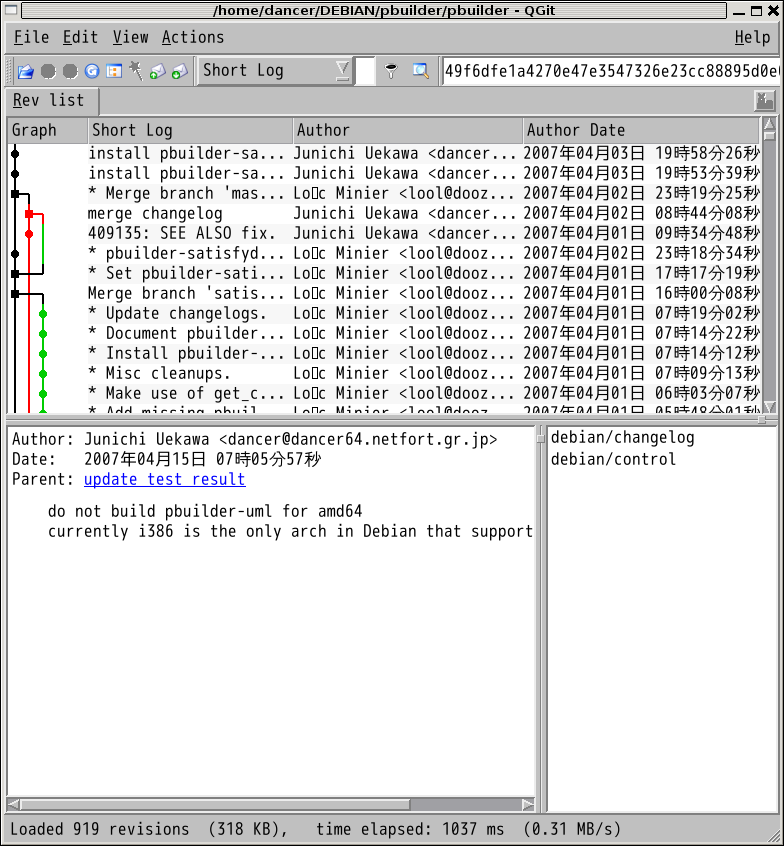
\includegraphics[width=0.8\hsize]{image200704/qgit.png}
\end{minipage}

\subsection{git-buildpackage の流れ}

git-buildpackage\footnote{apt-get install git-buildpackage でインストー
ル可能} を利用した場合のパッケージングの流れを紹介します。前提として、 
upstream では謎の利用不可能なSCMを利用して開発をすすめており、Debian
Developerはリリース毎に出てくる tar-ball しか利用できないものとします。

\includegraphics[width=1\hsize]{image200704/git-buildpackage.eps}

\subsubsection{git-import-dsc}

まず、Debian Developerはアップストリームの tarball を展開し、
そこで dh\_{}makeを実行し、一連のパッケージング作業を行います。

\begin{commandline}
[14:10:52]dancer64:work> cp ../upstream/vvv-0.1.tar.gz .
[14:10:57]dancer64:work> 
[14:11:03]dancer64:work> tar xfz vvv-0.1.tar.gz 
[14:11:08]dancer64:work> cd vvv-0.1
[14:11:12]dancer64:vvv-0.1> dh_make -f ../vvv-0.1.tar.gz 

Type of package: single binary, multiple binary, library, kernel module or cdbs?
 [s/m/l/k/b] s

Maintainer name : Junichi Uekawa
Email-Address   : dancer@debian.org 
Date            : Sat, 14 Apr 2007 14:11:28 +0900
Package Name    : vvv
Version         : 0.1
License         : blank
Type of Package : Single
Hit <enter> to confirm: 
Done. Please edit the files in the debian/ subdirectory now. You should also
check that the vvv Makefiles install into $DESTDIR and not in / .
[14:14:44]dancer64:vvv-0.1> debuild -us -uc 
 fakeroot debian/rules clean
dh_testdir
dpkg-buildpackage (debuild emulation): full upload (original source is included)
Now running lintian...
W: vvv: binary-without-manpage usr/bin/hello-world.sh
W: vvv: script-with-language-extension usr/bin/hello-world.sh
E: vvv: helper-templates-in-copyright
E: vvv: description-is-dh_make-template
W: vvv: wrong-bug-number-in-closes l3:#nnnn
E: vvv: section-is-dh_make-template
Finished running lintian.
[14:16:51]dancer64:vvv-0.1> cd ..

[14:17:42]dancer64:work> ls
vvv-0.1		vvv_0.1-1.diff.gz  vvv_0.1-1_amd64.build    vvv_0.1-1_amd64.deb
vvv-0.1.tar.gz	vvv_0.1-1.dsc	   vvv_0.1-1_amd64.changes  vvv_0.1.orig.tar.gz
\end{commandline}

すると、Debianのソースパッケージファイルなどができます。

git-import-dsc は dsc ファイルをオプションにとると、[パッケージ名]ディレ
クトリを作成し、その中に git のローカルレポジトリを作成し、upstream と master ブラ
ンチ(通常利用するブランチ)を作成し、upstreamにアップストリームのツリーを
入れ、master に debian への改変を加えた後のツリーを入れます。この状態で、
git-buildpackage などでパッケージがビルドできる状態になっています。

\begin{commandline}
[14:17:42]dancer64:work> git-import-dsc vvv_0.1-1.dsc 
Upstream version: 0.1
Debian version: 1
Initialized empty Git repository in .git/
Created initial commit b7e3ddd5bb1033c2cd9ae90d86ea8b6f55fb34be
 3 files changed, 16 insertions(+), 0 deletions(-)
 create mode 100644 Makefile
 create mode 100644 hello-world.sh
 create mode 100755 orig.sh
dpkg-source: warning: extracting unsigned source package (/home/dancer/tmp/git-test/work/vvv_0.1-1.dsc)
dpkg-source: extracting vvv in /home/dancer/tmp/git-test/work/tmpwJLVOR/unpack/vvv-0.1-1
dpkg-source: unpacking vvv_0.1.orig.tar.gz
dpkg-source: applying /home/dancer/tmp/git-test/work/vvv_0.1-1.diff.gz
 VCSCMD:  git
LOGTEXT Imported vvv-0.1-1
into Git repository

Created commit 041935d50363f69bcb7ff1b5e0df43b79784b6b1
 9 files changed, 149 insertions(+), 2 deletions(-)
 create mode 100644 debian/README.Debian
[中略]
 create mode 100755 debian/rules
[14:17:58]dancer64:work> cd vvv
[14:18:09]dancer64:vvv> git-status
# On branch master
nothing to commit (working directory clean)
[14:18:12]dancer64:vvv> git-branch
* master
  upstream
\end{commandline}

\subsubsection{git-import-orig}

新しいアップストリームのバージョンがリリースされた場合には、
git-import-dsc で作成されたディレクトリの中で git-import-orig コマンドを
実行して、ローカルレポジトリにインポートします。

\begin{commandline}
[14:18:50]dancer64:vvv> git-import-orig ../../upstream/vvv-0.2.tar.gz -u 0.2 
Upstream version is 0.2
Repository has uncommitted changes, commit them first: 
# On branch master
# Untracked files:
#   (use "git add <file>..." to include in what will be committed)
#
#	build-stamp
#	configure-stamp
#	debian/files
#	debian/vvv/
nothing added to commit but untracked files present (use "git add" to track)

[14:19:04]dancer64:vvv> debclean 
Cleaning in directory ./.git/refs/tags
Directory ./.git/refs/tags: contains no debian/changelog, skipping
Cleaning in directory .
dh_testdir
dh_testroot
rm -f build-stamp configure-stamp
# Add here commands to clean up after the build process.
/usr/bin/make clean
make[1]: ディレクトリ `/home/dancer/tmp/git-test/work/vvv' に入ります
make[1]: `clean' に対して行うべき事はありません.
make[1]: ディレクトリ `/home/dancer/tmp/git-test/work/vvv' から出ます
dh_clean 
[14:19:28]dancer64:vvv> git-import-orig ../../upstream/vvv-0.2.tar.gz -u 0.2 
Upstream version is 0.2
Importing ../../upstream/vvv-0.2.tar.gz to upstream branch...
Switched to branch "upstream"
  master
* upstream
 VCSCMD:  git
LOGTEXT Imported vvv-0.2
into Git repository



Created commit 8e61554f99a28de9b10c23ae0319b8cc4aa07b40
 2 files changed, 4 insertions(+), 1 deletions(-)
 create mode 100644 NEWS
Merging to master
Switched to branch "master"
* master
  upstream
 100% (14/14) done
Auto-merged Makefile
CONFLICT (content): Merge conflict in Makefile
Automatic merge failed; fix conflicts and then commit the result.
git-pull returned 1
Couldn't pull upstream to .
Import of ../../upstream/vvv-0.2.tar.gz failed
[14:19:50]dancer64:vvv> cat Makefile 
all:

install:
<<<<<<< HEAD:Makefile
	install -o root -g root -m 755 hello-world.sh $(DESTDIR)/usr/bin/hello-world.sh
=======
	install -o root -g root -m 755 hello-world.sh /usr/local/bin/hello-world.sh
>>>>>>> 8e61554f99a28de9b10c23ae0319b8cc4aa07b40:Makefile

clean:

.PHONY: all install clean

[14:19:58]dancer64:vvv> vi Makefile
[14:20:15]dancer64:vvv> git-commit -a -m '0.2 debian changes'
Created commit cffcdabb818fdacc38f1a21bab744c56480d1a44
\end{commandline}

この操作により、upstream ブランチに新しいバージョンがインポートされ、
master ブランチに変更がマージされ、適切なタグが作成されます。

\subsubsection{git-buildpackage}

各種編集を行い、コミットを完了したら、git-buildpackage を実行し、レポジ
トリの内容から Debian パッケージを作成します。--git-tag オプションを付け
ておくとビルドしなおしたら適切なタグを自動でつけてくれるので便利です。
また、コミットしわすれていると警告を出してくれるのもよいです。

\begin{commandline}
[14:21:26]dancer64:vvv> git-buildpackage 
[中略]
You have uncommitted changes in your source tree:
# On branch master
# Changed but not updated:
#   (use "git add <file>..." to update what will be committed)
#
#	modified:   debian/changelog
#
no changes added to commit (use "git add" and/or "git commit -a")

Use --git-ignore-new to ignore.
[14:21:34]dancer64:vvv> git-commit -a -m 'update changelog'
Created commit 98ae75017264f86192d30b894191d862b98821f5
 1 files changed, 6 insertions(+), 0 deletions(-)
[14:21:43]dancer64:vvv> git-buildpackage 
dh_testdir
dh_testroot
rm -f build-stamp configure-stamp
[中略]
$ git-buildpackage -us -uc --git-tag
\end{commandline}
%$

\subsection{アップストリームが git で管理している場合}

別のシナリオを考えてみます。アップストリームが git で管理している場合に
直接 git を利用したワークフローは幾分か簡単にできます。
どちらがよいかはわかりませんが、参考までに掲載します。

git-clone したらローカルレポジトリはリモートレポジトリから見たらただのブランチ
のため、ローカルレポジトリで変更を加えていれば、
git-pull するたびにアップストリームの変更をマージすることになります。
ビルドする際には、debuild などを直接使えばよいでしょう。ただ、
この場合は自動でタグをつけたりはしてくれません。

\begin{commandline}
$ debuild -us -uc -i -I 
\end{commandline}
%$

そのため、git-import-dsc, git-import-orig を使わない場合においても
git-buildpackage を利用するのがよいでしょう。upstream ブランチが必要にな
るのは git-import-orig をする際だけなので、master ブランチのみしかなく
ても動きます。

\begin{commandline}
$ git-buildpackage -us -uc -i -I 
\end{commandline}

\includegraphics[width=1\hsize]{image200704/git-clone.eps}

\dancersection{git の実装技術的解説}{上川 純一}

簡単にgit のレポジトリ\footnote{ローカルレポジトリもリモートレポジトリも
基本的には同じファイル構成です。}のファイル構成のコンセプトを紹介します。
レポジトリのファイルは .git ディレクトリ以下\footnote{もしくは環境変数 
GIT\_{}DIR で指定された場所}にあります。基本的なオブジェクトは commit,
tree, blob の三種類があります。.  git/objects/ 以下にファイルはgzip 圧縮
された状態で保存されています。.  git/HEAD (最近は 
.git/refs/heads/master) に最新の commit のハッシュ(ハッシュはデータの
sha1sumをとることで取得している)が記録されています。commit の中身を見る
と、tree のハッシュと 親 commit とコミットメッセージ情報が含まれています。
treeを見ると、そのコミットのときのディレクトリ情報が含まれており、それぞ
れのファイル実体(blob)の hash 値が含まれています。

なお、objects はばらばらで管理されるとディスクの利用効率が悪いので
git-repack コマンドを利用して pack 形式で保存されることが多いです。そう
なると、.git/objects/pack に保存されます。

\includegraphics[width=0.38\hsize]{image200704/git-filesystem-concept.eps}
\includegraphics[width=0.5\hsize]{image200704/git-filesystem-concept2.eps}

この情報を具体的にコマンドラインで確認してみた例を例示します。特に重要な
点は、'head'ファイルへの書き込みというOS観点ではアトミックに実装できるオ
ペレーションでコミットが実現されているということでしょう。\footnote{ファ
イルの SHA-1 ハッシュ値の衝突が発生しないということが前提です。ただ、現
実的に問題になることは無いでしょう。}

\begin{commandline}
[11:39:25]dancer64:pbuilder> cat .git/refs/heads/master
49f6dfe1a4270e47e3547326e23cc88895d0e05d
[11:39:38]dancer64:pbuilder> git-cat-file -t 49f6dfe1a4270e47e3547326e23cc88895d0e05d
commit
[11:39:44]dancer64:pbuilder> git-cat-file commit 49f6dfe1a4270e47e3547326e23cc88895d0e05d
tree 98dc4f51c0ae895607db43f8b617a7cacfbdc34b
parent e40c851b3017b09a609e2e36af6ae8a20b8ffff3
author Junichi Uekawa <dancer@dancer64.netfort.gr.jp> 1176588357 +0900
committer Junichi Uekawa <dancer@dancer64.netfort.gr.jp> 1176588357 +0900

do not build pbuilder-uml for amd64
currently i386 is the only arch in Debian that supports user-mode-linux
[11:39:47]dancer64:pbuilder> git-cat-file -t 98dc4f51c0ae895607db43f8b617a7cacfbdc34b
tree
[11:39:52]dancer64:pbuilder> git-cat-file tree 98dc4f51c0ae895607db43f8b617a7cacfbdc34b|strings|head -5
100644 .cvsignore
100644 .gitignore
100644 AUTHORS
o[v'a
R100644 COPYING
[11:40:13]dancer64:pbuilder> git-ls-tree 98dc4f51c0ae895607db43f8b617a7cacfbdc34b|head -5
100644 blob 99ee691a57a1d79999965e8f9362da79d18e8ce4    .cvsignore
100644 blob e4e5f6c8b2deb54bf38312dd9e2f53489b60d6a6    .gitignore
100644 blob 30ded29ac4176f5b7627618b27a8cb15c7ea0a52    AUTHORS
100644 blob b7b5f53df1412df1e117607f18385b39004cdaa2    COPYING
100644 blob 97cae37dd0355d4f29837bc02bbad4bcdba98914    ChangeLog
[11:40:18]dancer64:pbuilder> git-cat-file -t 97cae37dd0355d4f29837bc02bbad4bcdba98914
blob
[11:40:36]dancer64:pbuilder> git-cat-file blob 97cae37dd0355d4f29837bc02bbad4bcdba98914|head
2007-04-11  Junichi Uekawa  <dancer@debian.org>

        * AUTHORS, etc: remove $Id$, which is CVS specific

2007-04-10  Junichi Uekawa  <dancer@debian.org>

        * Documentation/pbuilder-doc.xml: update documentation

        * pbuilder-modules: say lenny instead of sarge

[11:40:43]dancer64:pbuilder> ls .git/objects/97/cae37dd0355d4f29837bc02bbad4bcdba98914
.git/objects/97/cae37dd0355d4f29837bc02bbad4bcdba98914
[11:40:58]dancer64:pbuilder> ls -l .git/objects/97/cae37dd0355d4f29837bc02bbad4bcdba98914
-r--r--r-- 1 dancer dancer 27255 2007-04-11 09:01 .git/objects/97/cae37dd0355d4f29837bc02bbad4bcdba98914
\end{commandline}


\dancersection{プロジェクトトラッカーの勧め}{矢吹 幸治(yabuki@netfort.gr.jp)}

\subsection{プロジェクトトラッカーとは何か}
プロジェクトトラッカーは、ある作業にかかった時間を記録するためのプログラムです。
\subsection{なぜトラッカーを使うのか}
このツールは、作業時間を計測するツールです。このトラッカーを使うことにより、

\begin{enumerate}
 \item 自分の能力を高める。
 \item ある作業を開始して完了するまでの時間を予想しやすくする。
 \item 自分の時間の使い方を見直すことができる。
\end{enumerate}

という利点があります。
欠点としては、自分の作業を{\large 記録するのがめんどくさい }という点があ
ります。{\large し
かし記録する利点に比べれば、かける手間は引き合います。}

また、他人に私を観察してもらうよりは、自分で私を観察するほうが、己の自尊
心のために安全です。--- 「他人に指摘してもらう」ことは多くの人にとって苦
痛で、受け入れ難い事です。

\subsection{Debian 4.0(“Etch”)で利用できるトラッカー(Tracker)は?}
以下の4つがある

\begin{itemize}
 \item  gnotime -- GTK ベース
 \item  karm -- Qt ベース
 \item  wmwork -- X ベース
 \item  worklog -- CUIベース
\end{itemize}

\subsubsection{gnotime}
\begin{wrapfigure}{r}{5cm}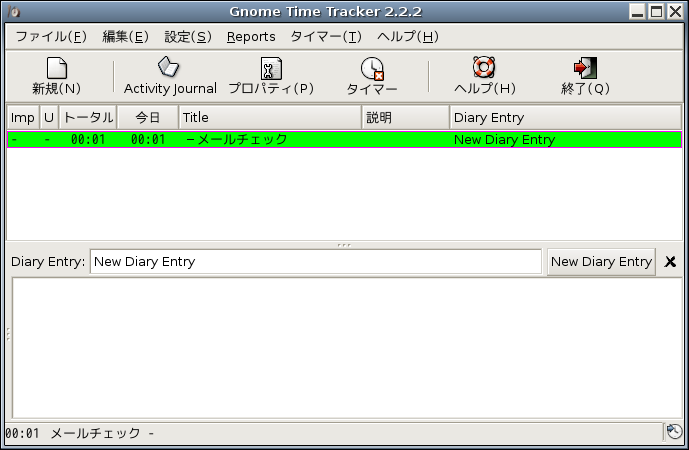
\includegraphics[width=5cm]{image200704/gnotime.png}\end{wrapfigure}
GTKで書かれた、GNOMEと親和性の高いプロジェクトトラッカー。
日本語も使えて、活動履歴(Activity Journal)も出力できる。DesktopでGNOMEを使っているなら、おすすめ。

\subsubsection{karm}
Qtで書かれたプロジェクトトラッカー。たぶん便利だと思う。今回は時間切れで試さず。私はKDE使いじゃないのでだれか、小ネタでいいので発表で使い勝手レポートをしてくれるとうれしい。
\subsubsection{wmwork}

Xがあれば動く、プロジェクトトラッカー。

\begin{wrapfigure}{r}{2cm}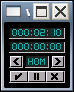
\includegraphics[width=2cm]{image200704/wmwork.png}\end{wrapfigure}

インストール方法は、

\begin{commandline}
 aptitude install wmwork
\end{commandline}

 Small is beautiful. シンプルで  Windowmaker や blackbox などのシンプ
ルなwindow manager と相性が良さそう。

設定は、wmworkが起動していないときに、~/.wmwork/wmworklogを編集する。詳細は、/usr/share/doc/wmwork/配下のドキュメントを参照せよ。以下は、/usr/share/doc/wmwork/exsample/worklogを引用した。

\begin{commandline}
 1# sample wmwork configuration file
 2# do not edit while wmwork is running
 3#
 4# you may save this file as an initial ~/.wmwork/worklog
 5
 6A02:0:comment here
 7PSI:0
 8TEST:0:only 'TES' will be shown
\end{commandline}

上記の設定ファイルをみると判るが、最初の 3 letter がwmworkの表示に使われる。識別子というべきか。また、この最初の部分に指定したファイル名でログが取られる。次に費した時間(秒単位)、最後にコメントである。

\verb!~/.wmwork/!以下にロックファイルができて、2重起動ができないようになっている。

\subsubsection{worklog}

\begin{wrapfigure}{r}{7cm}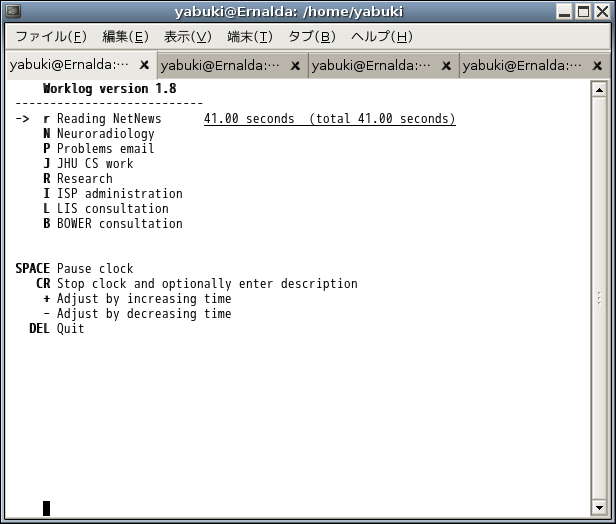
\includegraphics[width=7cm]{image200704/worklog.png}\end{wrapfigure}

CUIで動かせる。sshなどでサーバに入って作業をしても、このプログラムなら利用できる。

\begin{commandline}
 aptitude install worklog
\end{commandline}

このプログラムには、起動するまでに設定ファイルを作成しておく必要がある。
詳しくは、/usr/share/doc/worklog/のファイル群を読むこと。設定ファイルの
書式は、

\begin{commandline}
 キー:割り当てる名前
\end{commandline}

です。例えば

\begin{commandline}
 B:BOWER consultation
 L:LIS consultation
 R:Research
 r:Read NetNews
\end{commandline}

であれば、B,L,R,rのキーで対象となる時間を切替えながら計測できます。残念
ながら表示には日本語(UTF-8)は通りません。(ログには日本語(UTF-8)がそのま
ま出ているのでlvなどでは読めました。

{\texttt /usr/share/doc/worklog/examples/projects}に
雛型ファイルがあるので、これをコピーして改変して使うのがよいでしょう。

\begin{commandline}
 alias wl='worklog $HOME/logs/worklog.projects $HOME/logs/worklog.time.log'
\end{commandline}

がお薦めのaliasだそうです。確かに、設定ファイルのキーバインド毎にログが
生成されるので、ディレクトリを作っておくのが良いでしょう。

\subsection{この資料のコピーライト}

この資料は、GPLで配布します。不明点などあれば、メールなどの手段で連絡を
ください。\footnote{矢吹 幸治(yabuki@netfort.gr.jp)
}

\dancersection{今後の計画}{上川 純一}

\begin{itemize}
 \item 5月:
 \item 6月:スコットランドで開催
 \item 7月:
 \item 8月:
 \item 8月:
 \item 8月:
 \item 8月:
 \item 12月:反省会
\end{itemize}

\cleartooddpage

\begin{minipage}[b]{0.2\hsize}
 \definecolor{titleback}{gray}{0.9}
 \colorbox{titleback}{\rotatebox{90}{\fontsize{80}{80} {\gt デビアン勉強会} }}
\end{minipage}
\begin{minipage}[b]{0.8\hsize}

\vspace*{15cm}
\hrule
\vspace{2mm}

\includegraphics[width=2cm]{image200502/openlogo-nd.eps}
\noindent \Large \bf Debian 勉強会資料\\ \\
\noindent \normalfont \debmtgyear{}年\debmtgmonth{}月\debmtgdate{}日 \hspace{5mm}  初版第1刷発行\\
\noindent \normalfont 東京エリア Debian 勉強会 (編集・印刷・発行)\\
\hrule
\end{minipage}

\end{document}
